% THIS IS SIGPROC-SP.TEX - VERSION 3.1
% WORKS WITH V3.2SP OF ACM_PROC_ARTICLE-SP.CLS
% APRIL 2009
%
% It is an example file showing how to use the 'acm_proc_article-sp.cls' V3.2SP
% LaTeX2e document class file for Conference Proceedings submissions.
% ----------------------------------------------------------------------------------------------------------------
% This .tex file (and associated .cls V3.2SP) *DOES NOT* produce:
%       1) The Permission Statement
%       2) The Conference (location) Info information
%       3) The Copyright Line with ACM data
%       4) Page numbering
% ---------------------------------------------------------------------------------------------------------------
% It is an example which *does* use the .bib file (from which the .bbl file
% is produced).
% REMEMBER HOWEVER: After having produced the .bbl file,
% and prior to final submission,
% you need to 'insert'  your .bbl file into your source .tex file so as to provide
% ONE 'self-contained' source file.
%
% Questions regarding SIGS should be sent to
% Adrienne Griscti ---> griscti@acm.org
%
% Questions/suggestions regarding the guidelines, .tex and .cls files, etc. to
% Gerald Murray ---> murray@hq.acm.org
%
% For tracking purposes - this is V3.1SP - APRIL 2009

% \documentclass{acm_proc_article-sp}
\documentclass{sig-alternate}

\pdfpagewidth=21cm
\pdfpageheight=29.7cm

% \usepackage{mathptmx}
\usepackage{microtype}
\usepackage{enumitem}
\usepackage[usenames,dvipsnames]{xcolor}
	\definecolor{bleudefrance}{rgb}{0.19, 0.55, 0.91}
\usepackage{tikz}

\setlength{\parindent}{15pt}
% \setlength{\parskip}{-0.5pt}

\def\sharedaffiliation{%
\end{tabular}
\begin{tabular}{c}}

\begin{document}

% --- Author Metadata here ---
\conferenceinfo{DLfM'14,}{September 12 2014, London, United Kingdom}
\CopyrightYear{is held by the owner/author(s).~Publication rights licensed to ACM.} % Allows default copyright year (20XX) to be over-ridden - IF NEED BE.
\crdata{978-1-4503-3002-2/14/09}  % Allows default copyright data (0-89791-88-6/97/05) to be over-ridden - IF NEED BE.
% --- End of Author Metadata ---


\title{Correcting Large-Scale OMR Data with Crowdsourcing}

\numberofauthors{1} 
\author{
\alignauthor
Charalampos Saitis, Andrew Hankinson, and Ichiro Fujinaga\\
       \vspace{4pt}
       \affaddr{Schulich School of Music, McGill University}\\
       \affaddr{Montreal, QC H3A 1E3, Canada}\\
       \vspace{4pt}
       \email{\{charalampos.saitis,andrew.hankinson\}@mail.mcgill.ca, ich@music.mcgill.ca}
}
% 
\maketitle
\begin{abstract}
This paper discusses several technical challenges in using crowdsourcing for distributed correction interfaces. The specific scenario under investigation involves the implementation of a crowd-sourced adaptive optical music recognition system (Single Interface for Music Score Searching and Analysis project). We envisage the distribution of correction tasks beyond a single workstation to potentially thousands of users around the globe. This will have the effect of producing human-checked transcriptions, as well as significant quantities of human-provided ground-truth data, which may be re-integrated into an adaptive recognition process, allowing an OMR system to ``learn'' from its mistakes. Drawing from existing crowdsourcing approaches and user interfaces in music (e.g., Bodleian Libraries) and non-music (e.g., CAPTCHAs) applications, this project aims to develop a scientific understanding of what makes crowdsourcing work, how to entice, engage and reward contributors, and how to evaluate their reliability. While results will be considered based on the specific needs of SIMSSA, such knowledge can be useful to a variety of musicological investigations that involve labour-intensive methods.
\end{abstract}

\category{H.3.4}{Information Storage and Retrieval}{Systems and Software}[Distributed systems]
\category{H.5.3}{Information Interfaces and Presentation}{Group and Organization Interfaces}[Collaborative computing]
\category{H.5.5}{Information Interfaces and Presentation}{Sound and Music Computing}[Systems]

\keywords{Optical music recognition, music notation, crowdsourcing, web applications, music score searching}

\newpage
\section{Introduction}

The Single Interface for Music Score Searching and Analysis (SIMSSA) project\footnote{http://simssa.ca} is a recently funded initiative to investigate the development of a fully searchable digital musical document collection, including document digitization, high-volume optical music recognition (OMR), large-scale symbolic search systems, and digital document display. The goal of SIMSSA is to teach computers to recognize the musical symbols in digitized notation and assemble the data on a single website, making online search and analysis of musical scores possible for the first time. Scholars and the general public will be able to consult millions of musical works in the blink of an eye, a task that would previously have required many lifetimes. Central to the SIMSSA project is the use of Web-based technologies to facilitate the development of online \emph{crowdsourcing} tools for the collection of large amounts of human-checked transcriptions. 

SIMSSA aims to integrate Gamera \cite{droettboom2003} and Aruspix \cite{pugin2008}, two major desktop open-source OMR software platforms, into a cloud-based environment. These systems are unique for their capacity to ``learn'' from their mistakes by using human corrections of misrecognized symbols to improve their recognition abilities over time, resulting in highly cost-effective digitization and recognition workflows \cite{pugin2007}. By making them browser-based, distributed proofreading and correction can be potentially performed by anyone with a web browser and an Internet connection, anywhere in the world, thereby allowing for a constantly-improving search and retrieval system, as well as for the collection of human-provided ground-truth data to further reduce the amount of error in the final product while maintaining a level of quality and efficiency beyond simple automatic recognition \cite{hankinson2012}. 

In the following sections we outline the prime challenges facing the design of the crowd-sourced, adaptive OMR system envisioned by the SIMSSA initiative, focusing on those related to the user engagement and assessment. This position paper is part of an ongoing research programme that aims to provide SIMSSA with a theoretical framework for developing effective crowdsourcing tools. 

\section{Background}

Humans are critical components for performing quality control in a pattern recognition process, correcting the inevitable errors that automated systems make and ensuring these errors do not compound themselves in subsequent workflow steps \cite{hankinson2012b,burlet2012}. Correction, however, can be very time, labour and cost intensive. In the case of optical character recognition (OCR)---the textual counterpart of OMR---some unique solutions have been developed, leveraging collective intelligence and the Web to help offset the costs of this task. The reCAPTCHA project \cite{ahn2008} has produced over 5 billion human-corrected OCR words by presenting the correction task as a spam-fighting challenge to prove that the user is a human and not an automated system. The Australian Newspapers Digitisation Project (ANDP) \cite{holley2009} has created a distributed correction system, where more than 9,000 volunteers have now corrected more than 12.5 million lines of text, with more corrections added all the time.

Both these examples are manifestations of crowdsourcing, a Web-enabled, distributed problem-solving model that has emerged during the past decade \cite{brabham2008}. Its technical and conceptual underpinnings of crowdsourcing lie at the intersection of collective intelligence, outsourcing and the Internet \cite{brabham2013,saxton2013}. A crowdsourcing system is a system where a large number of people, known as contributors, are enlisted to help solve a problem defined by the system owners (corporations, libraries, researchers, etc.), which would normally require intensive (and often tedious), costly labour. Apart from helping reaching out to potentially thousands of users around the globe, the Internet offers a high degree of automation and unique possibilities for user management (e.g., wiki, discussion groups) \cite{doan2011}. Ever since the term was coined in 2006 \cite{howe2006nourl}, many names (citizen science, crowd wisdom, human computation, etc.), definitions \cite{arolas2012} and typologies \cite{geiger2011} of crowdsourcing have appeared in an attempt to provide this new concept with a theoretical framework. 


\section{Challenges}

Unlike small-scale public engagement activities such as tagging or rating a song, crowdsourcing requires a greater level of commitment from the contributor in terms of effort, time and intellectual input, as well as continuous assessment and reward by the system owners \cite{holley2010}. 

\textbf{How to engage contributors?} According to Doan, Ramakrishnan, and Halevy \cite{doan2011}, one can either \emph{require users} (e.g., students may be required to help correct transcriptions as part of the class curriculum), \emph{make users ``pay'' for service} (i.e., \emph{implicit} contribution; e.g., reCAPTCHA \cite{ahn2008}), \emph{piggyback on the user traces} (e.g., search query logs may be used for spelling corrections \cite{ahmad2005} or keyword generation \cite{fuxman2008}), or simply \emph{ask for volunteers}. For the latter a strategy to motivate individuals to contribute is required. To this end, methods and topics from the uses and gratifications theory can provide a useful framework for understanding intrinsic (e.g., fun, challenge, community) and extrinsic motivating factors (e.g., class assignment, practical reward) \cite{brabham2013}. 

\textbf{What type of tasks can users perform?} Many contributors may be hesitant at the prospect of re-editing an entire score, therefore it is necessary to ``chunk'' up error correction of an entire OMR corpus into much smaller units of work such as a single page, line or bar. In addition, different tasks may require different levels of musicological knowledge (e.g., notation systems) and thus be assigned to appropriate subgroups of contributors. For example, musicologists specializing in early music notation may perform more complex correction tasks (e.g., replacement of incorrect neumes) than volunteers with little or no relevant background (e.g., position and pitch of single notes). A two-stage strategy for crowd management is therefore needed, both prior to the assignment of the first task (using test tasks and/or questionnaires) and following the evaluation of previously assigned tasks (which may gradually increase the abilities of a contributor \cite{shen2003}).  

\textbf{How to evaluate users and their contributions?} Crowdsourcing, as with any open call to an undefined group of people, is prone to incompetent and sometimes malicious use. Continuous evaluation of users and their contributions is essential in monitoring individuals' abilities and thus assuring effective crowd management. A manual approach to this challenge includes the further distribution of contributions by ordinary users to an independent team of trusted users, whereby ``bad'' work is flagged on message boards \cite{doan2011}. For example, the same task can be assigned to three contributors. If one result differs substantially from the other two, then that contributor gets flagged. The less flags a contributor has, the more trustworthy he is. Such reliability testing can also be done on the fly; a contributor can be given a correction task for which the system already knows the solution, then flagged as reliable or unreliable based on their response \cite{doan2011}.    

\textbf{How to reward and retain users?} Provided that the contributions of a user are reliable, a strategy to reward and retain them should be encouraged. Such a strategy should be part of the overall crowd engagement approach (e.g., extrinsic motivation). For example, contributors may be offered exclusive beta versions of certain (possibly relevant) software or free access to digital libraries. Ideas may also be drawn from the emerging area of \emph{gamification} \cite{deterding2011}: contributors can earn badges that they can then redeem as points in online games; high-volume data collection and verification can be turned into a game where participants are rewarded points for their work (e.g., the ESP game \cite{ahn2004}; MajorMinor \cite{mandel2008}). 


\begin{figure}[t]
\begin{center}%\fontsize{8}{8}
\begin{tikzpicture}[
  source/.style={align=center,rounded corners,draw=black,fill=gray!10,text width=2.4cm,minimum height=1.1cm,font=\fontfamily{phv}\selectfont},
  empty/.style={align=center,fill=white,text width=4cm,minimum height=0.5cm,font=\fontfamily{phv}\selectfont,text=bleudefrance},
  fig/.style={align=center}]

% \node[empty] (platform) at (0,5) {Platform};

\node[source] (corpus) at (-2,5) {OMR \\ corpus};
\node[fig] (tasks) at (-2,2.5) {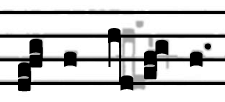
\includegraphics[scale=0.35]{figures/score-detail.png}};
% \node[source] (tasks) at (-2,2.5) {Individual tasks};
	\draw[->,thick] (corpus) -- (tasks);
\node[empty] (decomposition) at (-2,3.75) {Task decomposition};

\node[empty,text width=2.9cm] (engagement) at (2,6.25) {Crowd engagement};
\node[source] (crowd) at (2,5) {Crowd};
\node[source] (orgcrowd) at (2,2.5) {Organized \\crowd};
	\draw[->,thick] (engagement) -- (crowd);
	\draw[->,thick] (crowd) -- (orgcrowd);
\node[empty,text width=2.9cm] (management) at (2,3.75) {Crowd management};

\node[source] (assignment) at (0,0) {Human-checked transcriptions};
\node[source] (quality) at (0,-2.5) {Quality \\control};
\node[source] (output) at (0,-5) {Output};
	\draw[->,thick] (tasks) -- (assignment);
	\draw[->,thick] (orgcrowd) -- (assignment);
\node[empty] (assignment0) at (0,1.25) {Task assignment};
	\draw[->,thick] (assignment) -- (quality);
	\draw[->,thick] (quality) -- (output);
\node[empty] (evaluation) at (0,-1.25) {User/contribution evaluation};
\node[empty,text width=1.8cm] (reward) at (2.95,-2.2) {User reward};
\node[empty] (combination) at (0,-3.75) {Contribution combination};
	\draw[->,thick,rounded corners,bleudefrance] (evaluation) -| (3.8,2) |- (management);
	% \draw[->,thick,rounded corners,dotted] (evaluation) edge[out=0,in=0] (management);
	\draw[->,thick,rounded corners] (output) -| (-4,2) |- (corpus);
	% \draw[-,thick,rounded corners] (output) edge[out=-180,in=-90] (-4,2);
	% \draw[-,thick,rounded corners] (-4,2) edge[out=90,in=-180] (corpus);
	\draw[->,thick,rounded corners,bleudefrance] (evaluation) -| (reward);
	\draw[<->,thick,rounded corners,bleudefrance] (reward) -| (4.2,2) |- (engagement);

\end{tikzpicture}
\end{center}
\caption{A framework for correcting large-scale OMR data with crowdsourcing. Adapted from Kittur et al.~\cite[Fig.~2]{kittur2013}. Workflow- and user-specific challenges are marked in light blue.}
 \label{fig:model}
\end{figure}

Based on these considerations, Fig.~\ref{fig:model} presents a framework for crowdsourcing OMR transcription corrections, adapted from the more general one proposed by Kittur et al.~\cite[Fig.~2]{kittur2013}. We have identified two major types of challenges in implementing such a system (light blue colour): workflow-specific (task decomposition, task assignment, contribution combination \cite{doan2011}) and crowd-specific (engagement, management, evaluation, reward). We aim to explore solutions to these issues based on both hypothetical and real-world scenarios such as the Bodleian Libraries at the University of Oxford (currently using the Zooniverse platform\footnote{http://www.zooniverse.org/} for crowdsourcing descriptions of newly digitized scores\footnote{http://www.whats-the-score.org/}) and Neon.js (a browser-based neume editor\footnote{http://ddmal.music.mcgill.ca/neon} \cite{burlet2012}). 

Large-scale music databases (e.g., songs, scores) are becoming increasingly central to musicological scholarship. We hope that our ongoing survey of crowdsourcing experiences and tools will result in essential infrastructure components for creating next-generation globally accessible digital music libraries for the future musicologist.


\section{Acknowledgments}

We would like to thank Gabriel Vigliensoni and Esteban Maestre for fruitful discussions. The SIMSSA project is funded by the Social Sciences and Humanities Research Council (SSHRC) of Canada. 

\bibliographystyle{abbrv}
\bibliography{crowds} 

\end{document}
